\section{Results}
We evaluated our models on data collected from the California Report Card between January 18th to April 20th.
We administered our reference survey through SurveyMonkey between March 8th and March 14th.
We consider a set of 1575 total participants from the CRC and a sample of 611 SurveyMonkey participants whose grading activity was as follows:\\[1\baselineskip]

{\centering\scriptsize
\begin{tabular}[!ht]{ l | r | r | r | l }
Issue & No Change & Change & Skip & Median \\
\hline
\hline
  \multicolumn{5}{l}{\textbf{CRC}}\\
  \hline
  Obamacare & 749 & 223 & 593 & B \\
  \hline
  K12 & 849 & 172 & 544 & C+ \\
  \hline
  College & 923 & 139 & 503 & C-\\
  \hline
  Immigration & 693 & 105 & 767 & C \\
  \hline
  Marijuana & 881 & 118 & 566 & C \\
  \hline
  Marriage Rights & 929 & 105 & 531 & B+\\
\hline
\hline
\multicolumn{5}{l}{\textbf{Reference}}\\
\hline
  Obamacare & 498 & - & 113 & B \\
  \hline
  K12 & 561 & - & 50 & C \\
  \hline
  College & 573 & - & 38 & C-\\
  \hline
  Immigration & 375 & - & 236 & C+ \\
  \hline
  Marijuana & 498 & - & 113 & C \\
  \hline
  Marriage Rights & 554 & - & 57 & B+
\end{tabular}\\[1\baselineskip]
}

For any given issue, between 10\% and 20\% of those who assigned grades registered a grade change.
In all, 556 out of the 1575 CRC participants changed their grades at least once (Figure \ref{change-1}).
We also found that the aggregate results of the reference survey matched the CRC nearly perfectly.
On only two issues (K12 and Immigration), we found a observed differences which were both less than a letter grade (+ or -).
In our evaluation of these two surveys, we will use the unit \emph{full letter grades}.
For example, one full letter grade corresponds to the difference between an A grade and a B grade. 
A difference of a + or - is represented as $\frac{1}{3}$ eg. B to B+ or B+ to A-, each $\frac{1}{3}$ corresponds to one value on the 13-point scale.

\begin{figure}[h]
\hspace*{-2em}
    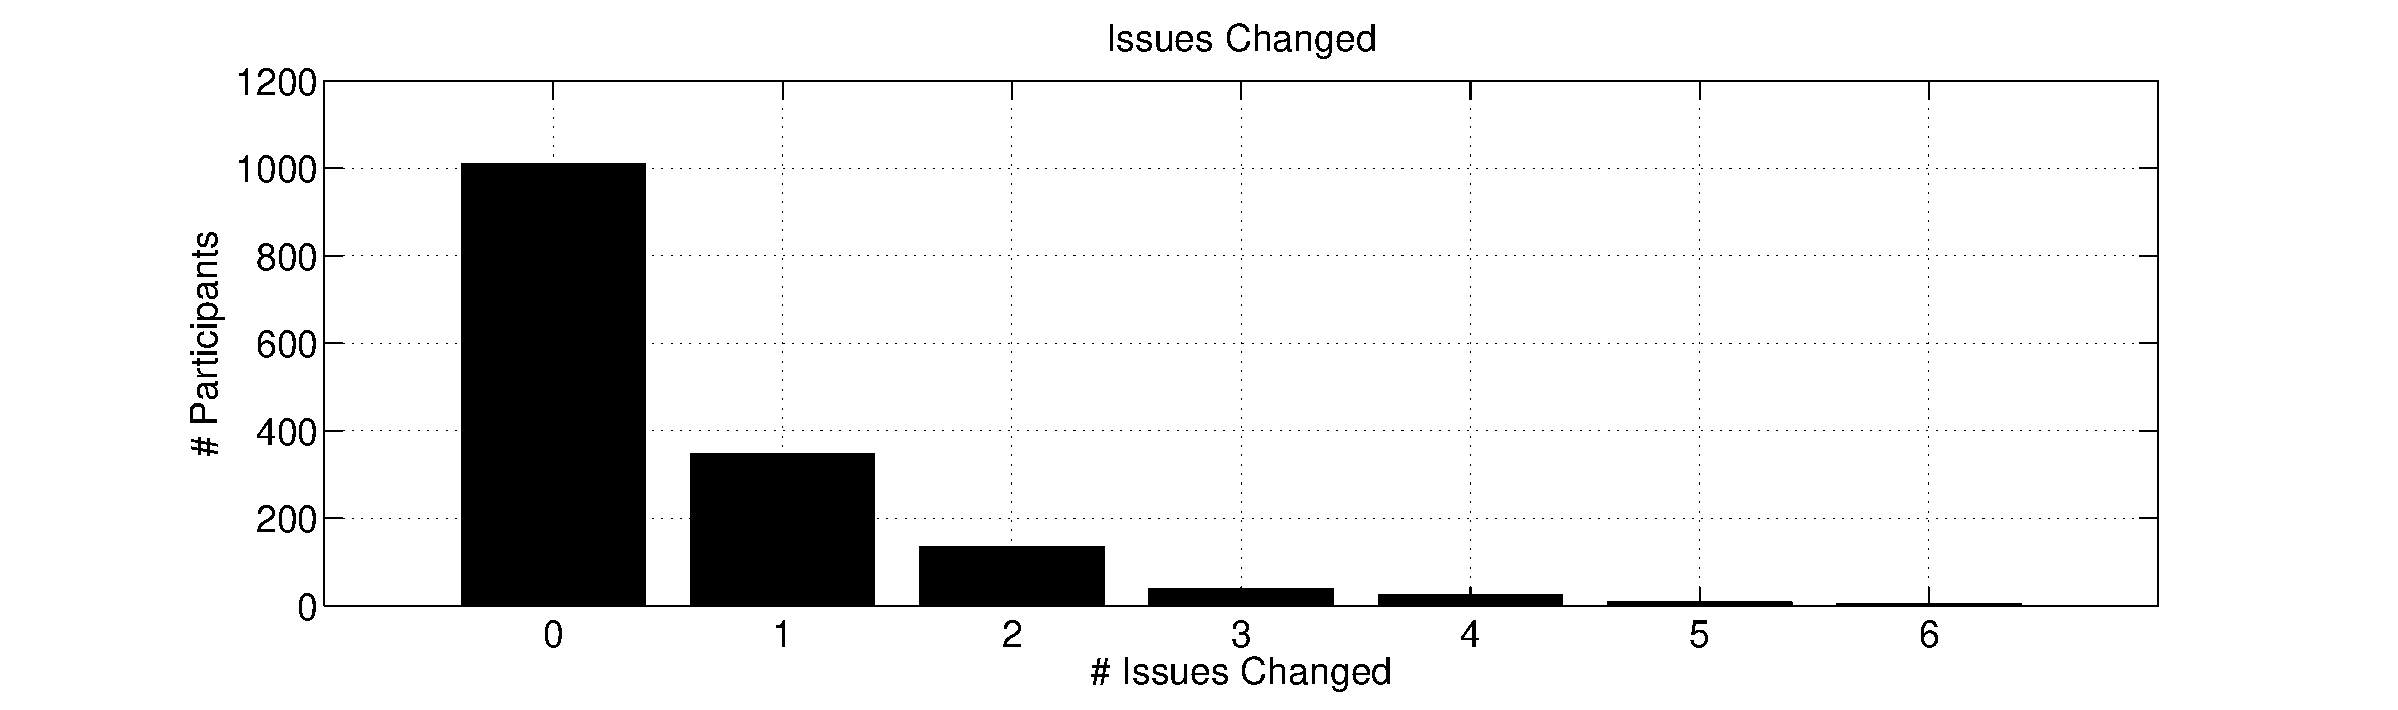
\includegraphics[scale=.25]{../plots/change-1.eps}
    \hspace*{-2em}
    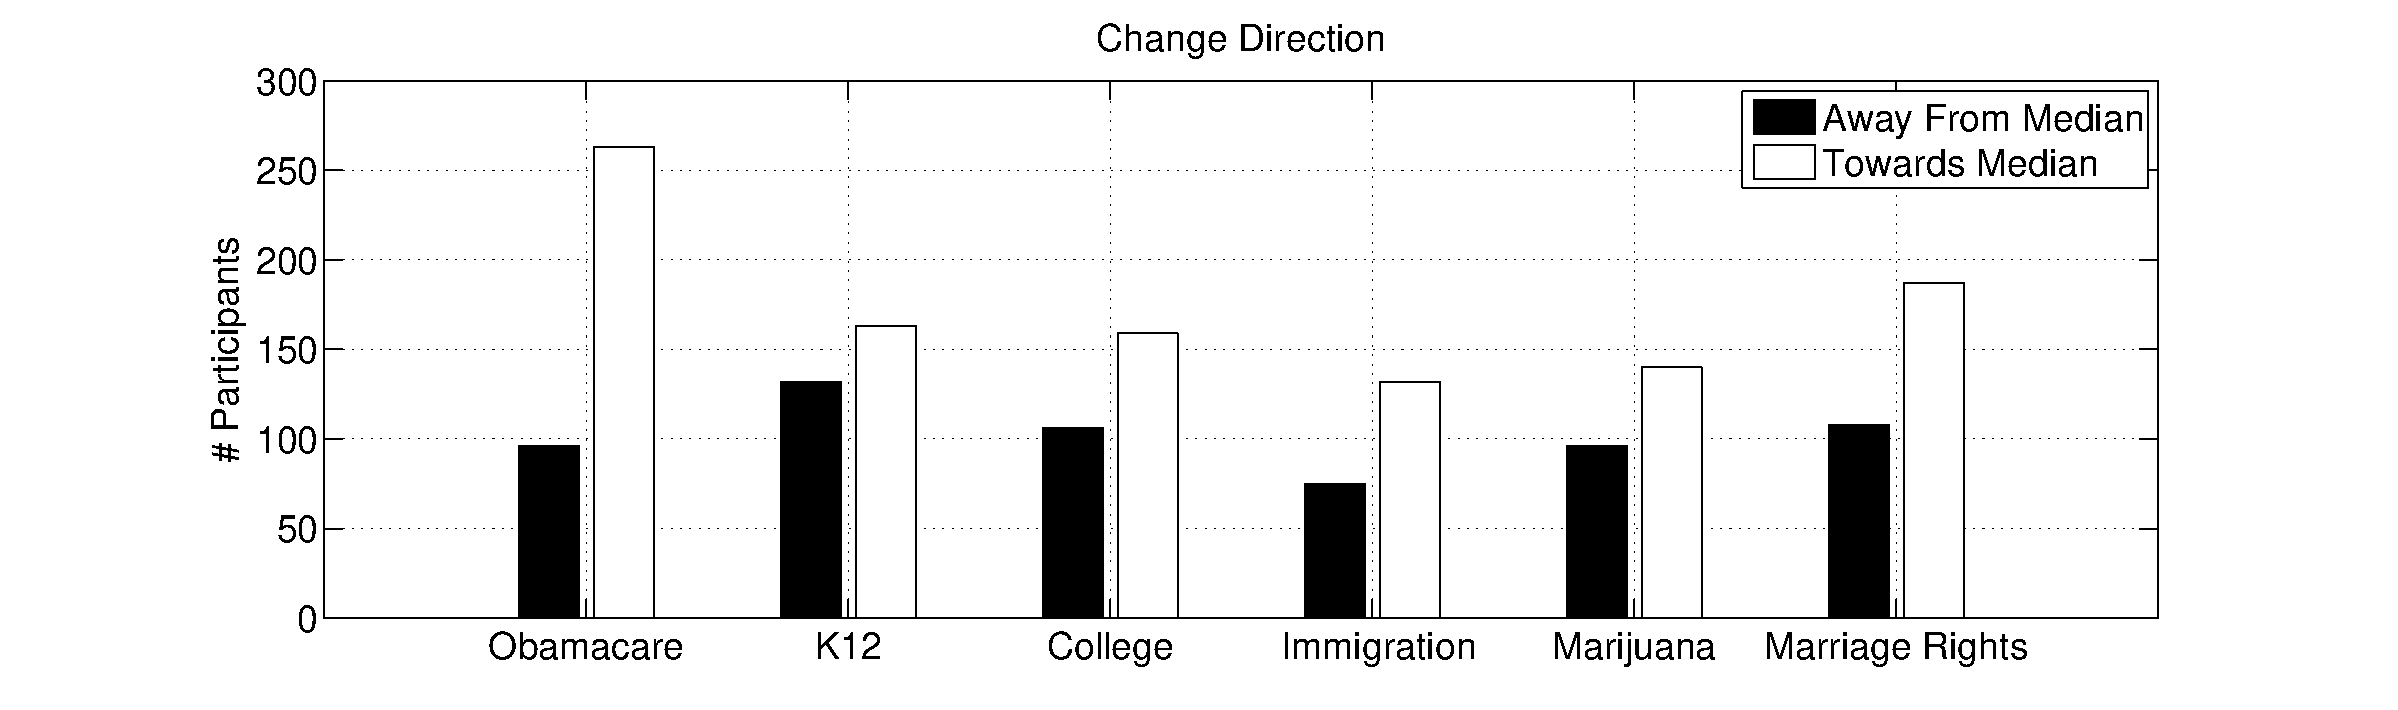
\includegraphics[scale=.25]{../plots/change-2.eps}
      \caption{The majority of participants did not change grades. 65\% change none of their grades, 22.0\% changed one, 8.6\% changed two, and only 6.5\% changed three or more. The lower figure shows that majority of grade changes were towards the median grade rather.}
      \label{change-1}
\end{figure}

\subsection{Moving Towards the Median}
Using the non-parametric test proposed in Section \ref{ht}, we tested the hypothesis of whether grade changes led to significantly more concentration around the median grade.
In our first experiment (Figure \ref{mdev-1}), we tested the absolute deviations of only the CRC participants.
We compared the group of participants that did not change their grades to the group that changed their grades.
We found that while there were no statistically significant differences between the initial grades of the two groups, the final grades of the group that changed were statistically significantly more concentrated than both their own initial grades and the grades of the no change group.
For the set of participants who changed their grades $P_c$ and those who did not $P_n$:
\begin{figure}[h]
\centering
    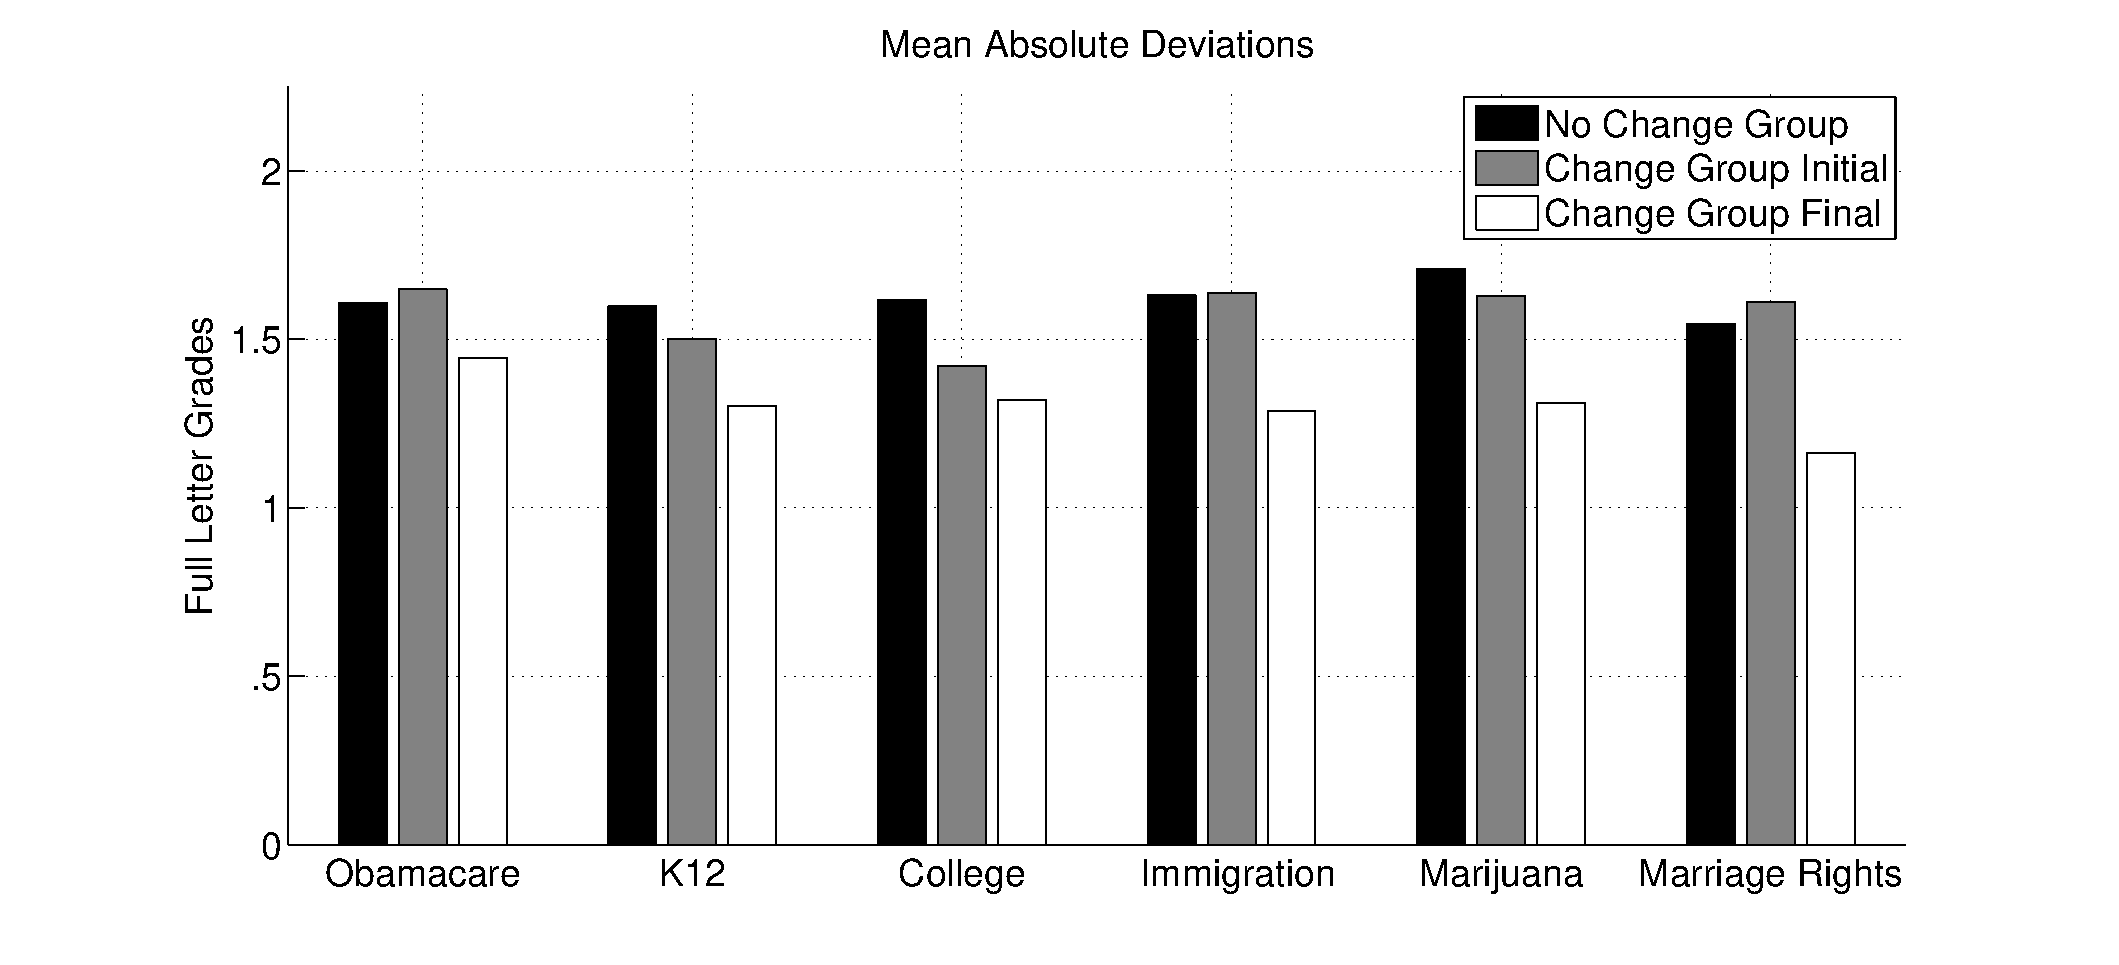
\includegraphics[scale=0.24]{../plots/abs-deviations-1.eps}
      \caption{For those participants that changed their grades, final grades were significantly more concentrated around the median grade than their initial grades. In addition, these grades are more concentrated than the grades for those who didn't change.}
      \label{mdev-1}
\end{figure}

{\centering
\scriptsize
\begin{tabular}[!ht] { r | r | r }
\label{dev-2}
  Issue & p-val($P_c$ vs. $P_n$) & p-val($i$ vs. $f$) \\
  \hline
  \hline
  Obamacare &  0.0286 & 0.0161 \\
  \hline
  K12 & 2.1314e-06 &  0.0086 \\
  \hline
  College & 1.3033e-04 & 0.0415 \\
  \hline
  Immigration & 7.3456e-07 &4.4170e-05\\
  \hline
  Marijuana & 2.7549e-10 & 4.2560e-05\\
  \hline
  Marriage Rights & 3.5946e-06 & 2.4644e-10 \\
\end{tabular}\\[1\baselineskip]
}

These results are consistent with social influence bias.
When participants change their grades, they are more likely to concentrate around the median.
What is particularly surprising is that the two groups of participants $P_n$ and $P_c$ are very similar in terms of initial grades, and the data suggests that a participant's susceptibility to social influence is not correlated with initial grades.

In our second experiment (Figure \ref{mdev-2}), we apply the same testing procedure to compare the grades from the CRC to to those in the reference survey.
We compare absolute deviations of the group of participants who changed their grades in the CRC against participants from the reference survey.
\begin{figure}[h]
\centering
    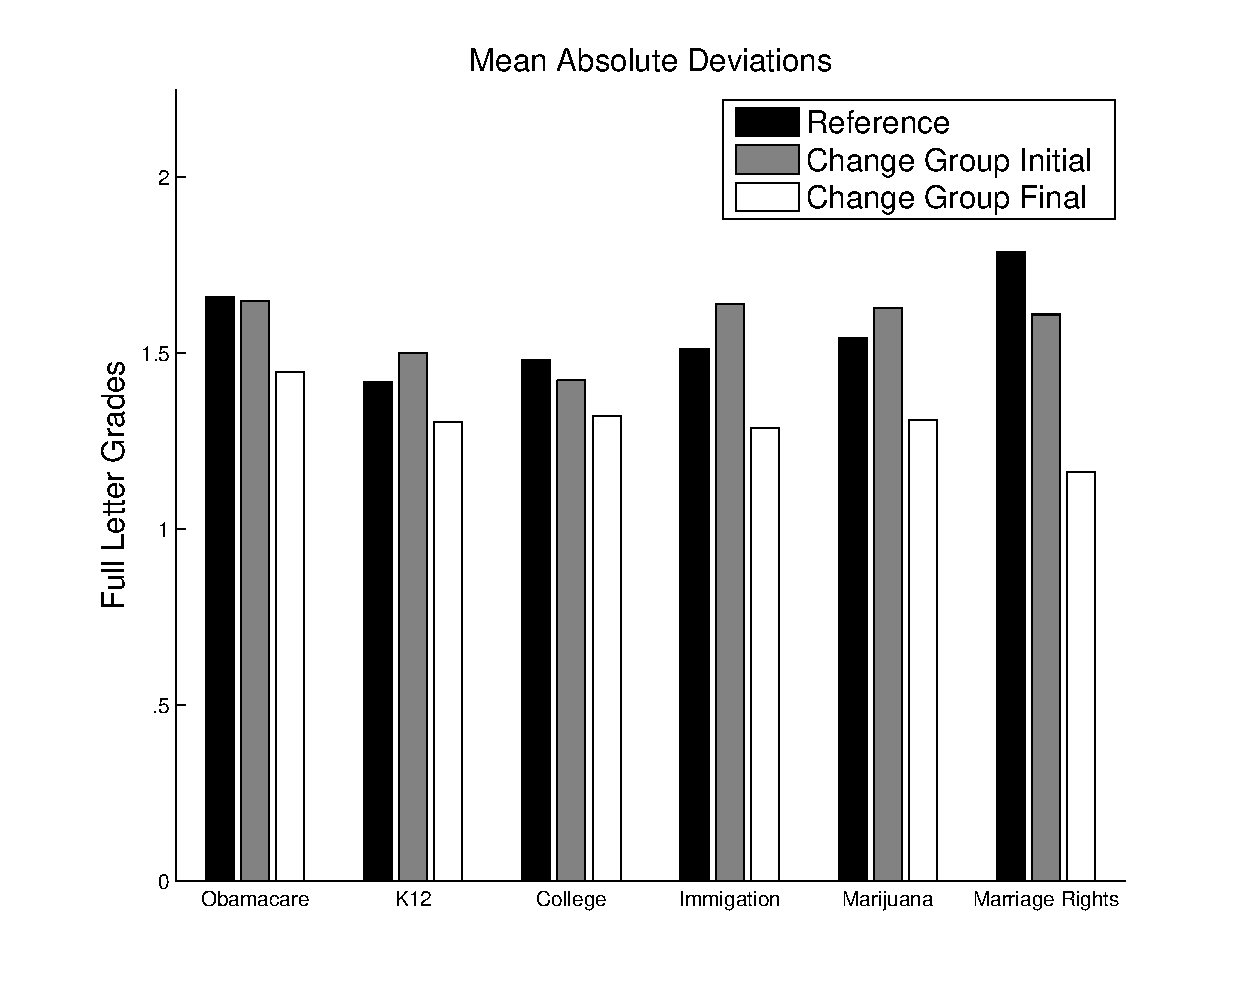
\includegraphics[scale=0.24]{../plots/bias-2.eps}
      \caption{We found that final grades were significantly more concentrated in the CRC compared to grades in the reference survey. Similar to Figure \ref{mdev-1}, we found that there was no statistically significant difference between the reference survey and the initial grades.}
      \label{mdev-2}
\end{figure}

{\centering
\scriptsize
\begin{tabular}[!ht] { r | r | r }
\label{ref-1}
  Issue & p-val($R$ vs. $i$) & p-val($R$ vs. $f$) \\
  \hline
  \hline
  Obamacare &  0.5386 & 0.0015 \\
  \hline
  K12 & 0.8283 & 0.0097 \\
  \hline
  College & 0.1452 & 0.0091 \\
  \hline
  Immigration & 0.3765 & 1.1787e-04\\
  \hline
  Marijuana & 0.7288 & 9.3111e-06\\
  \hline
  Marriage Rights & 0.2478 & 0.0161 \\
\end{tabular}\\[1\baselineskip]
}

The results of our two experiments are consistent with social influence bias.
We not only found that participants' changed grades were statistically significantly more likely to concentrate around the median, they were also more likely in comparison to the reference survey.
While correlation does not imply causation, we argue that this evidence rejects the null hypotheses and is most consistent with \textbf{Hypothesis 1}.
As the CRC was not a randomized survey, there are possibly confounding covariates eg. participants who changed their grades were more likely to leave tightly concentrated grades in the first place.
However, our comparison with the reference survey, and discovery that initial grades were largely consistent with the reference survey and with those that didn't change their grades, suggest that these confounding covariates are not very significant.
These results are encouraging and we hope to run a randomized participant study to confirm a causal relationship.

\subsection{Correlation vs. Absolute Deviation}
\label{exp-robust}
We ran an experiment to illustrate the problems of using correlation instead of absolute deviation.
In this experiment, we iterated through the initial grades each of participants in the change group $P_c$.
For each grade, we randomly sampled a final grade from group $P_n$.
In this model, since we sample final grades from the no change group, we know that the social influence bias hypothesis is not true.
However, when we calculate the correlation coefficient between $g_f[j] - m[j]$ and $g_i[j] - m[j]$, we find statistically significant correlations.

{\centering
\scriptsize
\begin{tabular}[!ht] { r | r | r }
\label{ref-2}
  Issue & corr & p-val \\
  \hline
  \hline
  Obamacare &  0.709 & 5.2e-56 \\
  \hline
  K12 & 0.659 & 4.73e-38 \\
  \hline
  College & 0.673 & 2.26e-36 \\
  \hline
  Immigration & 0.704 & 2.95e-32\\
  \hline
  Marijuana & 0.689 & 1.42e-34\\
  \hline
  Marriage Rights & 0.679 & 3.27e-41 \\
\end{tabular}\\[1\baselineskip]
}
There is a natural tendency for grades to group around the median grade and the correlation coefficient does not account for this.
However, if we measure the absolute deviation, we will find there is no statistically significant difference between the absolute deviations since they are sampled from the same group.
\subsection{Estimating the Social Influence Bias}
\begin{figure}[ht!]
\centering
    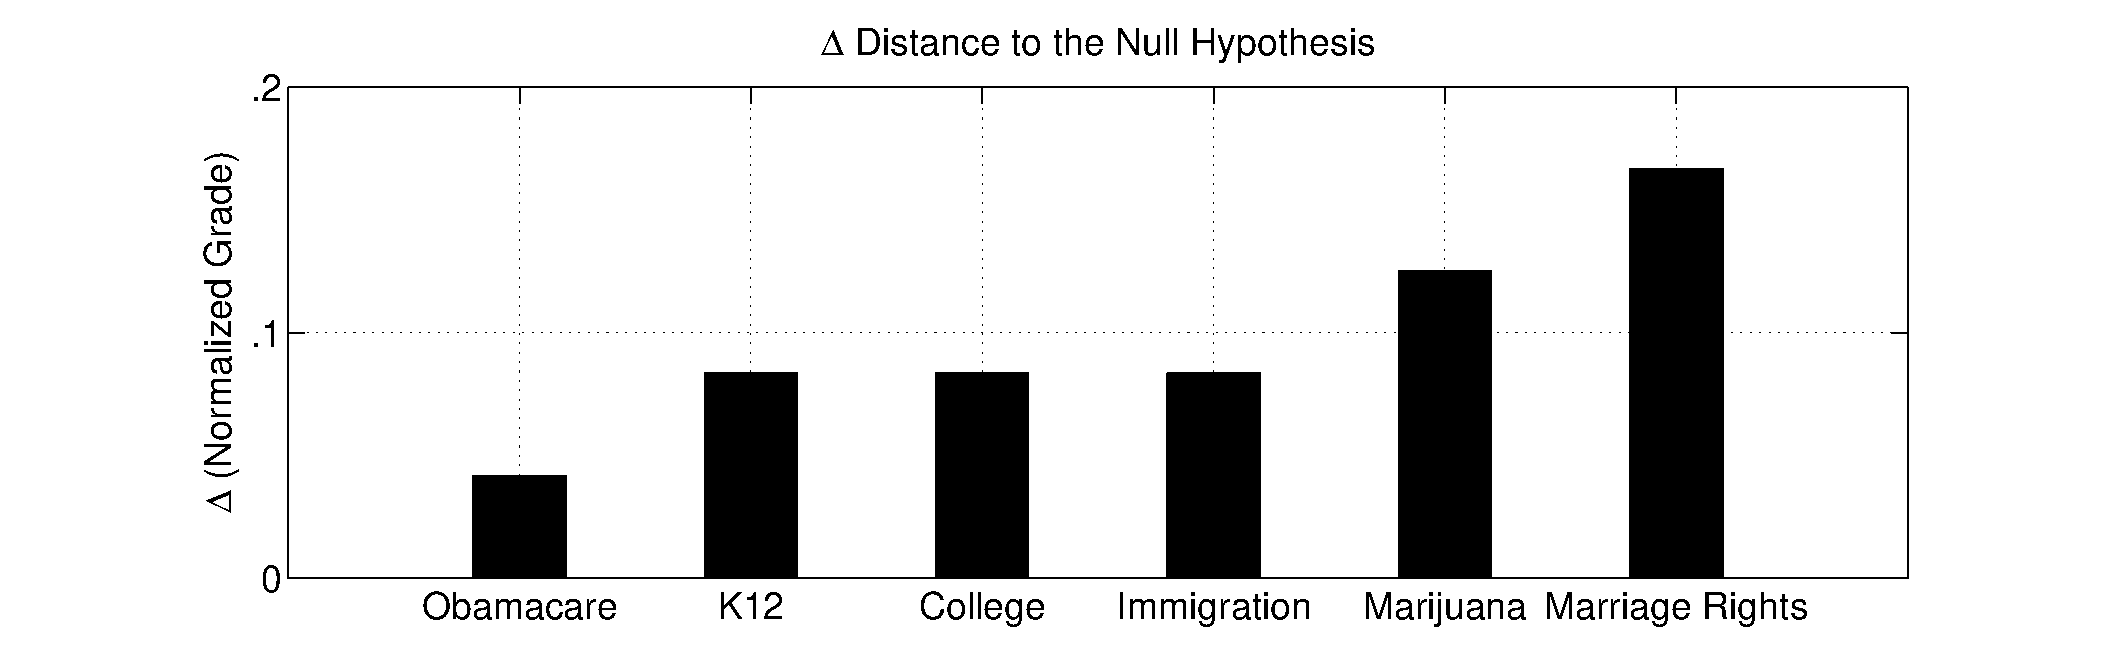
\includegraphics[scale=0.22]{../plots/shift-parameter.eps}
      \caption{We calculate the shift-parameter $\Delta$ which is the distance from the null hypothesis. Over all issues, we found that on average grades were more than 1/3 of a letter grade closer to the median.}
      \label{shift-1}
\end{figure}
We tested the hypotheses and conclude significant additional concentration of grades around the median grade.
In Section \ref{ht}, we described how we could use the results of the hypothesis test to estimate the $\Delta$ parameter, which quantifies how different the hypothesis is from the null distribution (no social influence bias).
We use $\Delta$ as a measure of social influence bias.

In Figure \ref{shift-1}, we show the parameter estimates for each of the issues.
As before, the units of the plot are in terms of letter grades.
For the issues about Marriage Rights, we find that parameter is 2/3 of a letter grade.
This means that the set of absolute deviations for the change group $X_c$ was on average 2/3 of a letter grade smaller.
For the other issues, the parameter was smaller indicating less of an effect of social influence bias.
On average over all issues, the grades were $0.3889$ full letter grades closer to the median, which corresponds to 8.9\% on a normalized absolute scale.

\subsection{Sequential Evolution of Social Influence}
Using the model proposed in Section \ref{path}, we calculated the test statistics for both the CRC and the Reference Survey.
Recall, that this model calculates the change in disagreement with the median; that is, how much did a participant disagree with the median on past responses compared 
to the current value.
A comparatively larger value in the CRC suggests repeated feedback of the median grade encourages future responses to be more moderate.
Figure \ref{path-1} illustrates the results of the experiment for the five last issues (K12, College, Immigration, Marijuana, Marriage Rights), and using the mean disagreement on the previous issues.
We see that for the last three issues the change in disgreement is comparatively much higher in the CRC.
The experimental results were not as significant as the other experiments and we found that only two issues Immigration (p=0.0037) and Marijuana (p=0.0287) showed an order dependence that was significantly greater than the reference survey.
In summary, we were not able to reject the null hypothesis for all issues, but we did find some indication that ordering plays an important role, at least for the later issues.

\begin{figure}[h]
	\centering
    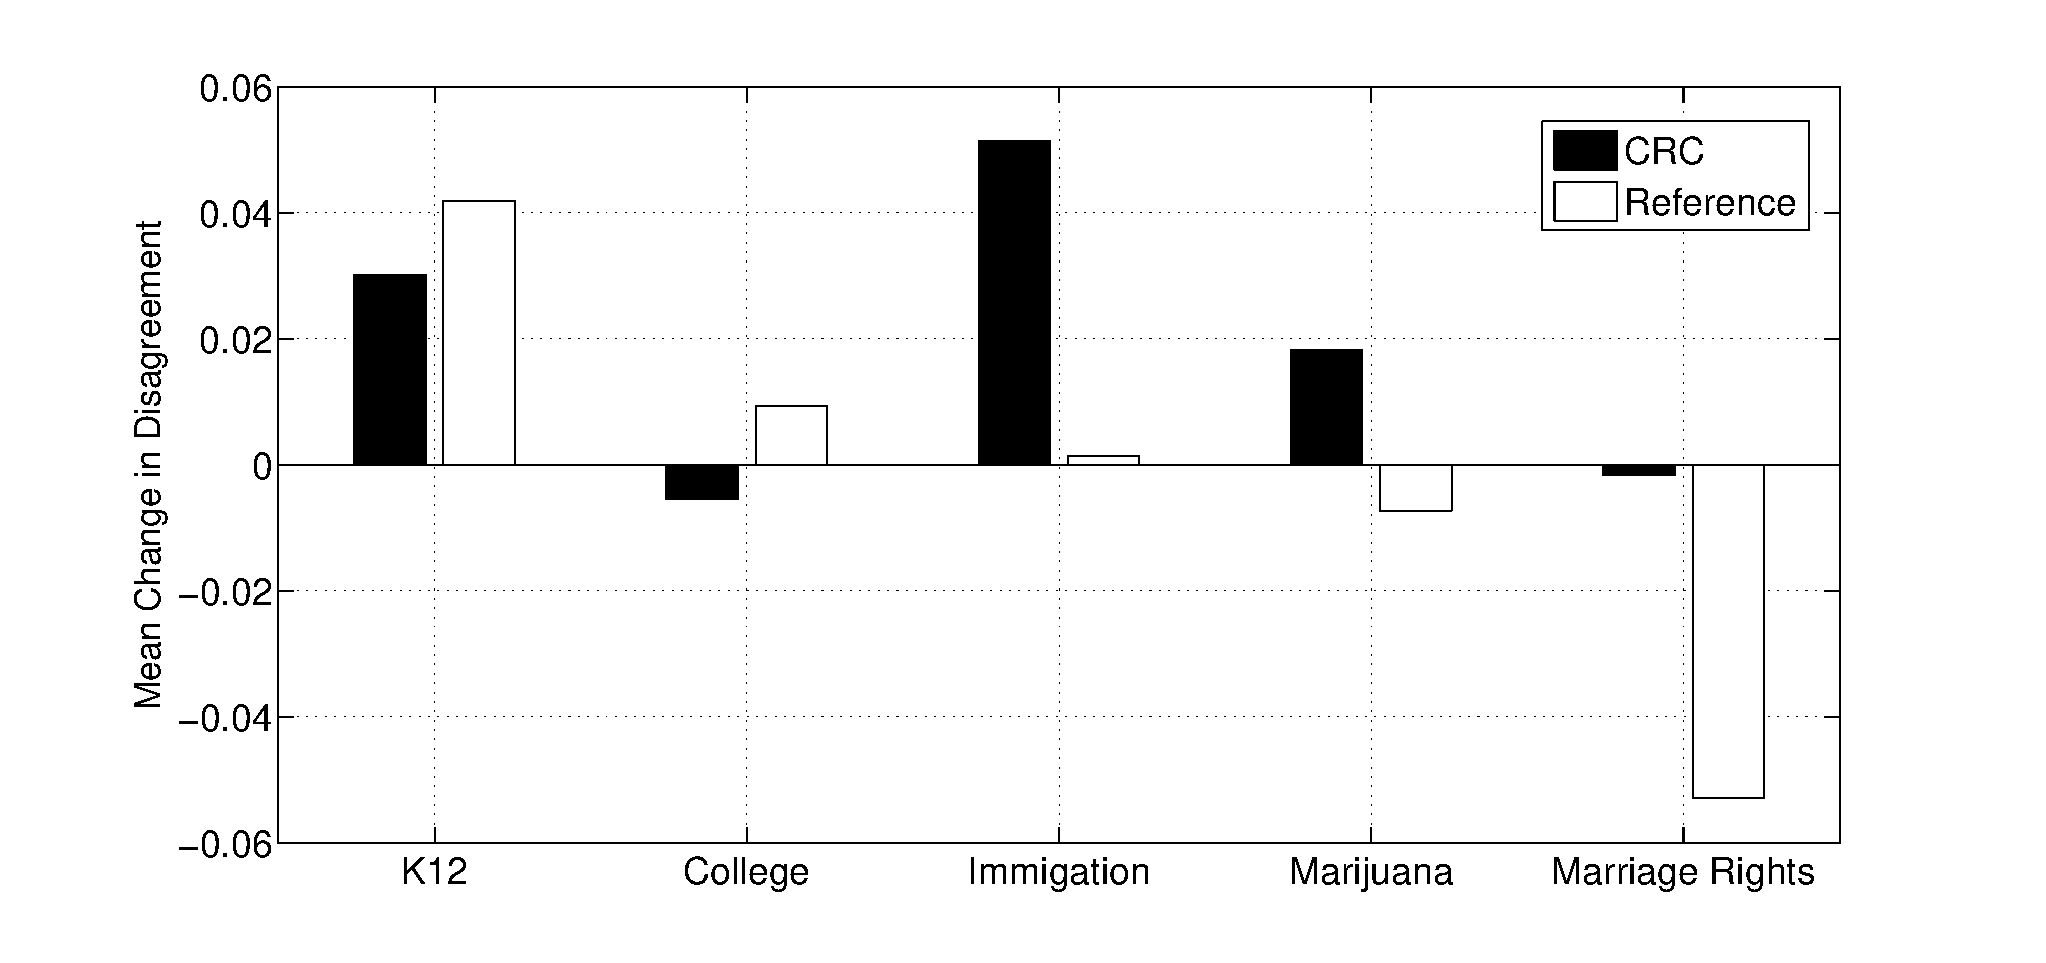
\includegraphics[scale=0.24]{../plots/path-dependence.eps}
      \caption{We measure the mean change in disagreement for each issue. The change in disagreement is defined as the average deviation with median on previous issues minus the deviation with the median on the current issue. We hypothesized that the CRC would have comparatively greater (or less negative) values than the reference survey.}
      \label{path-1}
\end{figure}

\begin{figure*}[ht!]
\hspace{-7em}
    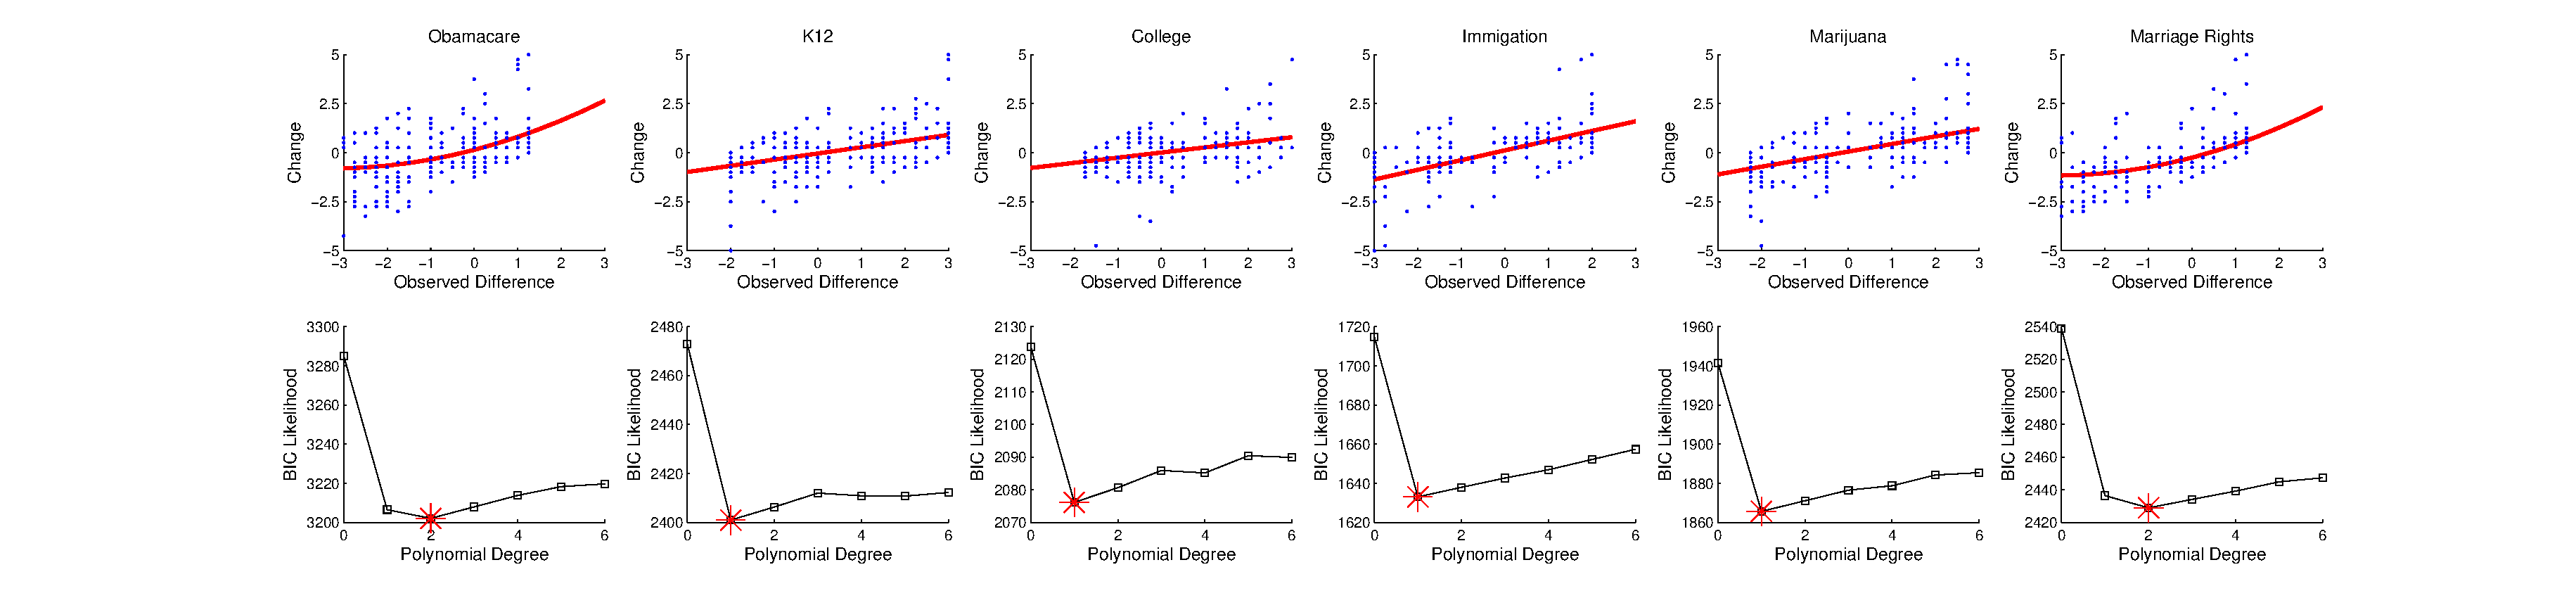
\includegraphics[scale=0.35]{../plots/BIC-optimization.eps}
      \caption{For the participants that changed their grades, we plot the difference between their grade and the median (X-axis), and their changed grade (Y-axis). We overlay the optimal polynomial model to represent the relationship $f(x) = y$. Below each plot, is the BIC objective function showing how we picked an optimal degree of polynomial.}
      \label{opt-1}
\end{figure*}
\subsection{Predicting Grade Changes}
We train the polynomial model proposed in Section \ref{changemod}, and the results are shown in Figure \ref{opt-1}.
Our model search and optimization through the BIC discovered that for four out of the six issues, K12, College, Immigration, and Marijuana, the model was linear.
This suggests homogeneity in positive and negative social influence effects for these issues.
What this implies is that on average participants who graded above the median and below the median moved towards the median with the same magnitude.
However, for Obamacare and Marriage Rights, we found that the relationship was quadratic.
Interestingly enough, over the domain of changes, the learned quadratic function was ``almost" linear, but with a steeper curve for grades above the median.
Participants who initially graded the state higher than the median had a more significant tendency to change downwards, in comparison to the upward tendency of those who graded less than the median.

These models further illustrate the subtlety and context dependence of social influence bias. 
In Muchnik et al. they observed a biasing tendency where both positive and negative influence led to increased upward bias (due to conforming and correcting tendencies respectively).
Compared to those results, our results are quite different as we observe movement towards the median for both positive and negative influences.

We also tested our model in terms of RMSE prediction error (Figure \ref{poly-1}). 
We held out 20\% of the pairs of ratings (observed change, actual) and tested the prediction error on this held out set.
We found that our model on average, over all issues, predicted final grade within $0.5150$ letter grades, or 11.8\% on a normalized absolute scale.
Note that 1/3 of a letter grade corresponds to the difference of just a + or - grade.

In a second experiment (Figure \ref{poly-1}), we applied the inverse model to infer initial grades from the final ones.
We measured the performance of the inverse model by re-caluating the $\Delta$, which can be interpreted as a distance from the null hypothesis of no social influence bias, for the predicted initial grades.
A $\Delta$ of 0 means that the null hypothesis of no social influence bias cannot be rejected, thus indicating perfect correction.
We found that there was on average a 76.3\% reduction in $\Delta$ which quantifies the concentration around the median. 
While the bias is still statistically significant, it is greatly reduced and the spread of participants around the median grade better reflects the initial grades.

\begin{figure}[h]
\hspace*{-2em}
    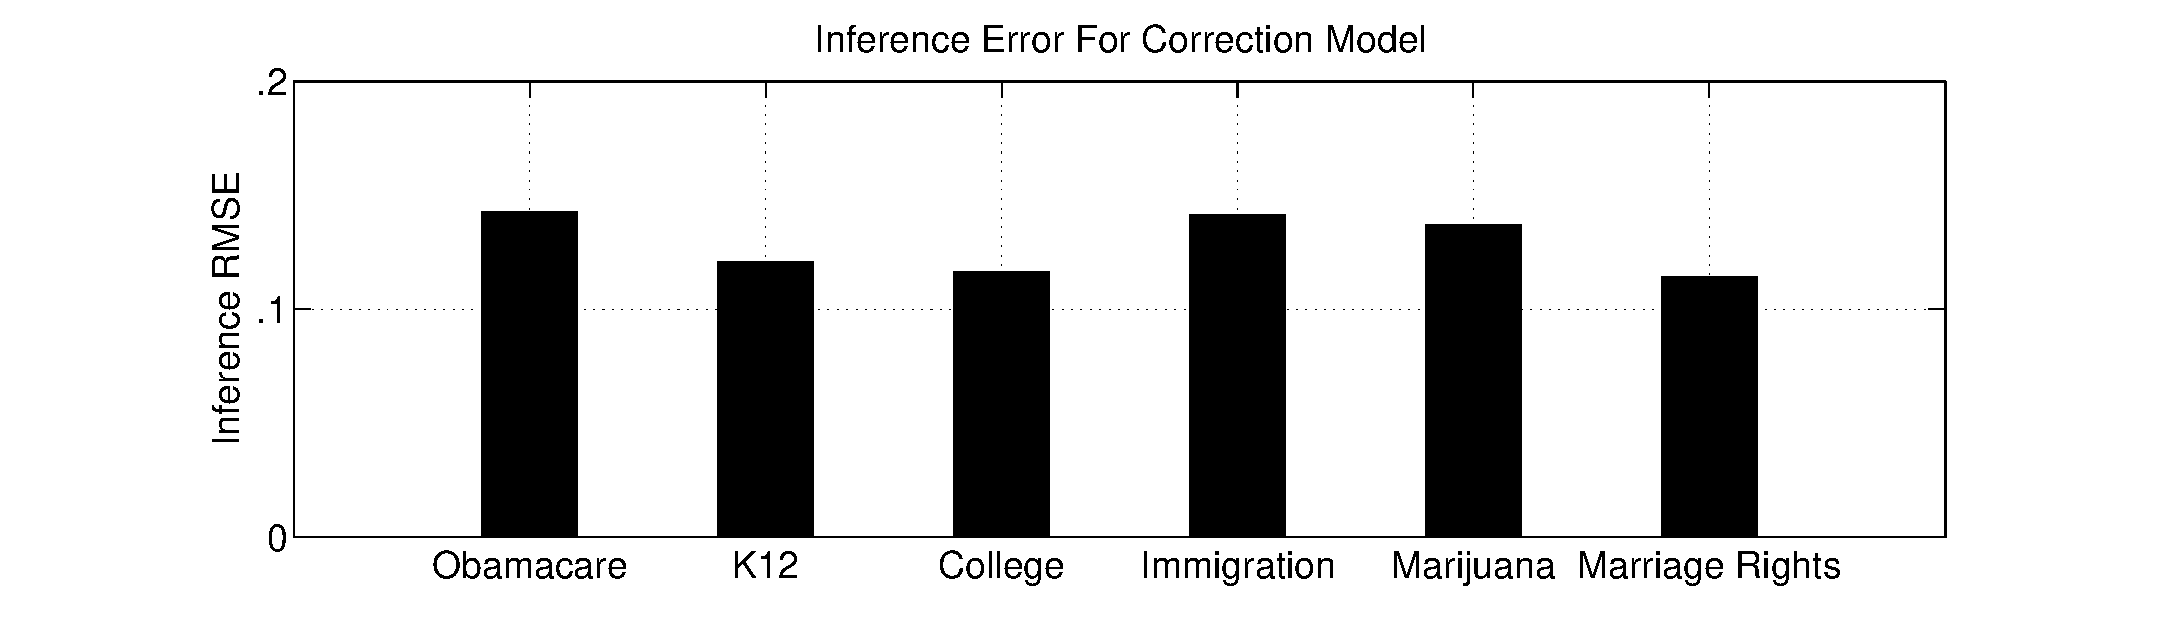
\includegraphics[scale=0.25]{../plots/prediction-error.eps}
    \hspace*{-2em}
    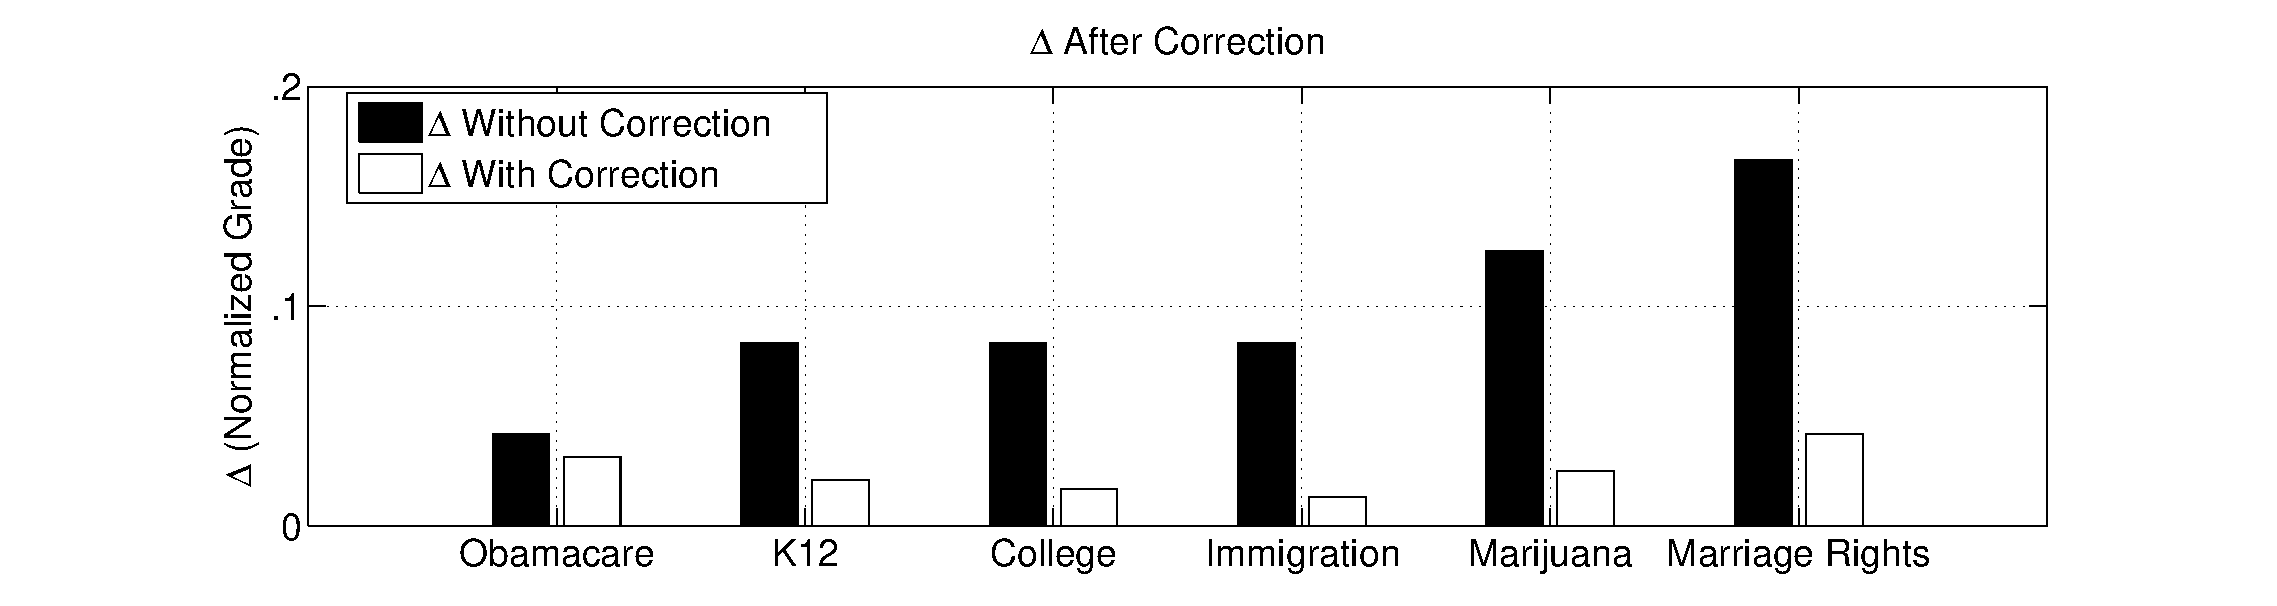
\includegraphics[scale=0.24]{../plots/shit-2.eps}
      \caption{We measured the RMSE prediction error of the polynomial model. We found that we could predict changes in all of the issues with less than 2/3 of a letter grade RMSE error. In the lower figure, we applied this model to correct for the social influence bias and found that, on average, we could reduce the effects by 76.3\%}
      \label{poly-1}
\end{figure}




